\documentclass{article}
\usepackage{graphicx} % Required for inserting images
\usepackage{hyperref} % Required for crosslink
\usepackage{subcaption} % Required for subcaption for figures
\usepackage{multirow} % Required for multirow in table
\usepackage{amsmath}
\usepackage{listings}
\usepackage{minted}
\usepackage{caption} % Required for left table name 
\usepackage{biblatex}
\usepackage{indentfirst}
\usepackage{pgfplots} % plot
\usepackage{xcolor}
\usepackage{placeins}
\usepackage{tikz}
\usepackage{fourier} 
\usepackage{array}
\usepackage{makecell}
\usepackage[colorlinks]{hyperref}


\addbibresource{ref.bib} 

\title{Parallelizing the Mandelbrot Set: CUDA Implementation Unveiling the Chaotic Beauty of Fractals}
\author{Mehmet Şamil Dinçer (2236248)\\
        Elvin Gültekinoğlu (2446169)}
\date{January 2024}

\begin{document}

\maketitle

\section{Abstract}
GPU computing is a new era of parallel computing, and it is commonly utilized in different solvers for several problems. The idea behind GPU programming is the same as that behind parallel programming. There are more GPU cores than CPU cores in a regular system; however, the main differences are communication between cores and the capacity of computations. If the same simple computation has to be calculated many times, GPUs are favorable, but if the computation load is heavy and cores have to be communicated to each other, then CPUs are favorable. One application of GPU programming is the parallelization of fractal computation in real and imaginary space. In this paper, this implementation is explained in detail, pointing out important characteristics of GPU. 





\clearpage
\section{Introduction}


Graphics processing unit (GPU) programming is a technique that allows for simultaneous processing of data by utilizing the computational capability of graphics processing units (GPUs) for tasks that are not related to graphics. In particular, NVIDIA created the CUDA programming framework, which stands for "Compute Unified Device Architecture," to make GPU programming simpler\cite{noauthor_cuda_nodate}. In CUDA computing, programmers make parallel algorithms called kernels that run on the GPU and use its many cores to do computations in parallel. The CUDA programming model allows seamless integration of CPU and GPU code, enabling developers to offload specific computational tasks to the GPU for accelerated processing. CUDA programming is extensively employed in scientific simulations, numerical computations, image processing, and machine learning to take advantage of the parallel architecture of GPUs. For specific categories of workloads, it provides substantial performance enhancements in comparison to conventional CPU-based methodologies. 

\begin{minipage}{0.45\textwidth}
    \centering
    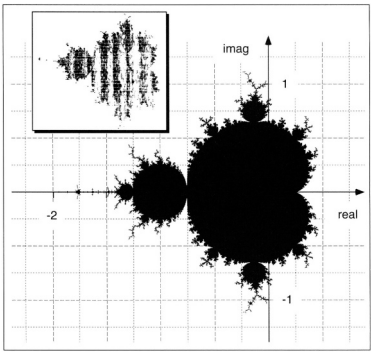
\includegraphics[width=1\textwidth]{Figures/mandelbrot.png}
    \captionof{figure}{The insert shows an original printout from Mandelbrot’s experiment. We have produced the large Mandelbrot set using a modern laser printer and a more accurate mathematical algorithm\cite{devaney_chaos_1989}}
    \label{mandel_brot_fig}
\end{minipage}%
\hfill
\begin{minipage}{0.45\textwidth}
    The Mandelbrot set is a complicated mathematical idea that comes from repeating a simple mathematical formula. The set is in the complex number plane, and each point is a complex number. It was named after Benoit B. Mandelbrot. Squaring the current value and adding the starting point are repeated steps in the iterative formula. The Mandelbrot set is made up of points that, after a given number of repetitions, do not escape to infinity. Together, these points create an incredibly complex and minutely detailed fractal pattern. The set demonstrates self-similarity across several scales, showcasing captivating and complicated geometric forms. Due to the stunning visual complexity that it possesses, the Mandelbrot set has become an iconic depiction of chaos theory and the beauty of complicated dynamical systems. It has captivated both mathematicians and amateurs alike\cite{devaney_chaos_1989}. The first try of mandelbrot fractals are  in Figure \ref{mandel_brot_fig}.
\end{minipage}


\clearpage
\section{The Theory and Methodology} 
This section extensively elaborates on the theoretical foundation, the approach used for GPU implementation through CUDA.

\subsection{Mandelbrot set }
The mandelbrot set calculation is very simple, but the output of the mandelbrot set is incredible. This calculation happened in 2D space. The x-axis is a real number, and the y-axis is an imaginary number.     


\begin{equation}  
    z_0 = 0 
    \label{MS_imp_eq_1}
\end{equation}
\begin{equation}  
    z_{n+1} = z_n^2 + c 
    \label{MS_imp_eq_2}
\end{equation}

The calculations are based on equations \eqref{MS_imp_eq_1} to \eqref{MS_imp_eq_2}, where \(z = x+yi\) and \(c = x_0 + y_0i\). Since both \(z\) and \(c\) have real and imaginary parts, they need to be simplified. The simplifications are shown in equations \eqref{MS_imp_eq_3} to \eqref{MS_imp_eq_7}.


\begin{equation}  
    z_{n+1} = z_n^2 + c -> x_{n+1} + y_{n+1}i = x_n^2 - y_n^2 + 2x_ny_ni +x_0 + y_0 
    \label{MS_imp_eq_3}
\end{equation}

\begin{equation}  
    x_{n+1} = \mathbb{R}(x_n^2 - y_n^2 + 2x_ny_ni +x_0 + y_0i )
    \label{MS_imp_eq_4}
\end{equation}

\begin{equation}  
    y_{n+1} = \Im(x_n^2 - y_n^2 + 2x_ny_ni +x_0 + y_0i )
    \label{MS_imp_eq_5}
\end{equation}

\begin{equation}  
    x_{n+1} = x_n^2 - y_n^2 +x_0  
    \label{MS_imp_eq_6}
\end{equation}

\begin{equation}  
    y_{n+1} = 2x_ny_n+ y_0
    \label{MS_imp_eq_7}
\end{equation}

After these simplifications are done, iteration can be done more easily. This iteration is repeated to choosing number of times. After every iteration, the \(z\) value has to be checked to see if \(z\) is still in range or going to infinity which means the calculation escaping number.  The next part is calculating the all \(c\) value in a desired range of 2D space. After every escaping of all \(c\) values is calculated, the next and last part is coloring. 
\clearpage 
\subsection{CUDA Implementation}
It is expected to implement GPU computing on a given serial code through CUDA to make it faster. This implementation is performed in Colab by connecting T4 GPU server since this environment enables working on cloud and running the code without any problem. Addition to these features, newly created files through the code are also obtained. \\

The most time-consuming, computationally intensive part in the serail code is "mandelbrot" function which performs the mandelbrot iteration in the complex plane by calling "tespoint" function. Testpoint function is another function on which the iteration number is returned to be used in further operations. Since these functions perform the same operation in a loop until the number of resolution in real and imaginary parts are reached, they constitutes the most time-intensive part of the code. \\

In Testpoint function, instead of complex numbers, an iterative relation for x and y is establised for the sake of computational simplicity. At that point, it is also important to note that x and y represents real and imaginary axes, respectively. The equations utilized for x and y are given in Equations \ref{cuda_imp_eq_1} and \ref{cuda_imp_eq_2}. Since this is aimed to be performed in an iterative manner, first y is calculated and then x is updated to be used as a new value in the next iteration. Later on, at the end of each iteration under the loop, the iteration number is returned. 

\begin{equation}  
    y = 2\times x_n \times y_n + y_0
    \label{cuda_imp_eq_1}
\end{equation}
\begin{equation}  
    y = x_n^2 - y_n^2 + x_0 
    \label{cuda_imp_eq_2}
\end{equation}

The Mandelbrot function performs iteration on a grid of numbers in the complex plane. The purpose of this is to record the iteration counts on an array by calling Tespoint functions. In other words, it uses the return of Testpoint function to store it in an array. \\

In order to perform GPU implementation, there are preliminary changes to be made. One of these changes is to create a device function which is designed to be executed on the GPU. The device function is called from within a CUDA kernel function which runs on the GPU and is designed to be executed in parallel by multiple threads. Considering the aforementioned explanations about the two functions forming the most time-consuming part of the code, Testpoint function is converted to device function while Mandelbrot function is converted to CUDA kernel. It should be noted that Testpoint function is called inside CUDA kernel which is the case mentioned in the definition. \\

The implementation of device function and CUDA kernel are provided below: 

\definecolor{mygray}{rgb}{0.95,0.95,0.95}
\begin{minted}[autogobble=true, frame=lines, framesep=4mm, baselinestretch=1.2, bgcolor=mygray, fontsize=\footnotesize, linenos=true, breaklines]{c}
__device__ int testpoint(complex_t c) {
    int iter;
    complex_t z = c;

    for (iter = 0; iter < MXITER; iter++) {
        // real part of z^2 + c
        double tmp = (z.x * z.x) - (z.y * z.y) + c.x;
        // update with imaginary part of z^2 + c
        z.y = z.x * z.y * 2.0 + c.y;
        // update real part
        z.x = tmp;
        // check bound
        if ((z.x * z.x + z.y * z.y) > 4.0) {
            return iter;
        }
    }
    return iter;
}

__global__ void mandelbrotKernel(int Nre, int Nim, complex_t cmin, complex_t dc, float *count){

  int m = threadIdx.x + blockIdx.x * blockDim.x;
  int n = threadIdx.y + blockIdx.y * blockDim.y;

    if (m < Nre && n < Nim) {
        complex_t c;
        c.x = cmin.x + dc.x * m;
        c.y = cmin.y + dc.y * n;
        count[m + n * Nre] = (float)testpoint(c);
    }
}
\end{minted}

In these functions, the main sections are left untouched and are the same with the ones in the serial code. However, there are little changes that have been made, especially in Kernel function. Since the Kernel function contains operations to be performed repeatedly, for loops in the original serial code are changed with one if statement instead of two to make the code faster. The conditions provided on the if statement for real and imaginary resolutions are provided through the global index of the current thread for x and y separately. These indices are calculated by the formulations in Equations \ref{cuda_imp_eq_3} and \ref{cuda_imp_eq_4} where threadIdx represents the index of the thread within its block along the x or y axis, blockIdx stands for the index of the block within the grid along the x-axis and blockDim is the size of a block along the x-axis. 

\begin{equation}  
    n = threadIdx.x + blockIdx.x * blockDim.x
    \label{cuda_imp_eq_3}
\end{equation}
\begin{equation}  
    n = threadIdx.y + blockIdx.y * blockDim.y
    \label{cuda_imp_eq_4}
\end{equation}

In these equations, the multiplication on the right calculates the offset of the current block in terms of the total number of threads that precede it along the x-axis. To complete the equation, current thread index is added and the global index is obtained. To illustrate this concept clearly, consider the representation given below. In this representation, B and T corresponds to block and thread, respectively. 

\begin{center}
    | B0 | B1 | B2 | B3 | B4 | ... |\\
    
    | T0 | T1 | T2 | T3 | T4 | ... |
\end{center}

Let's say blockDim is three for the sake of simplicity to illustrate the concept. Then the following calculations are made for global indices and results are obtained. The same procedure is applied on CUDA kernel also for both axes. \\

\begin{center}
    For T0 in B1: m = 0 + 1 * 3 = 3\\
    
    For T1 in B1: m = 1 + 1 * 3 = 4
\end{center} 

After device and Kernel functions are created,it can be proceed to the main part of GPU implementation which consists of ten steps. These steps are given below. 

\begin{enumerate}
\color{black}
\item Allocating device array: An array is allocated on the device which includes the GPU processor. 
\label{item_1}
\item Allocating memory on device array with cudaMalloc function. 
\label{item_2}
\item Creating events: To measure the computational time, start and end events are created. 
\label{item_3}
\item Calculating number of thread-blocks and threads per thread-block: Since the problem is in 2-D, this operation is performed for both axes. The number of threads per thread block (B) is chosen as 16 for x and y. The number of thread blocks to use (G) is calculated as given in Equation \ref{cuda_imp_eq_5} separately for x and y. In this equation, number of elements is the resolution specified at the beginning. 

\begin{equation}  
    \frac{Number of elements + B - 1}{B}
    \label{cuda_imp_eq_5}
\end{equation}

\label{item_4}
\item Recording start event: To calculate elapsed time later, timing is started. 
\label{item_5}
\item Launching the CUDA Kernel: The configuration parameters such as block and grid dimensions specified in Item \ref{item_3} are set up. 
\label{item_6}
\item Inserting end record event in stream: Timing is ended. 
\label{item_7}
\item Copying from the GPU back to the host: Results of computations performed on GPU are retrieved. 
\label{item_8}
\item Calculating and printing out elapsed time: The elapsed time is calculated and converted to seconds to be printed out. 
\label{item_9}
\item Freeing arrays: Created device array becomes free. 
\label{item_10}
\end{enumerate}

All of these steps are crucial in GPU programming with CUDA. Following these steps, a serial code is converted into a parallel one so the computational time reduces significantly. The finalized code is given below. 

\definecolor{mygray}{rgb}{0.95,0.95,0.95}
\begin{minted}[autogobble=true, frame=lines, framesep=4mm, baselinestretch=1.2, bgcolor=mygray, fontsize=\footnotesize, linenos=true, breaklines]{c}
%%cu
/*******************************************************************************
To compile: gcc -O3 -o mandelbrot mandelbrot.c -lm
To create an image with 4096 x 4096 pixels: ./mandelbrot 4096 4096
*******************************************************************************/
#include <math.h>
#include <stdio.h>
#include <stdlib.h>
#include <time.h>
#include "cuda.h"

int writeMandelbrot(const char *fileName, int width, int height, float *img, int minI, int maxI);

#define MXITER 1000

/*******************************************************************************/
// Define a complex number
typedef struct {
  double x;
  double y;
}complex_t;

__device__ int testpoint(complex_t c) {
    int iter;
    complex_t z = c;

    for (iter = 0; iter < MXITER; iter++) {
        // real part of z^2 + c
        double tmp = (z.x * z.x) - (z.y * z.y) + c.x;
        // update with imaginary part of z^2 + c
        z.y = z.x * z.y * 2.0 + c.y;
        // update real part
        z.x = tmp;
        // check bound
        if ((z.x * z.x + z.y * z.y) > 4.0) {
            return iter;
        }
    }
    return iter;
}

__global__ void mandelbrotKernel(int Nre, int Nim, complex_t cmin, complex_t dc, float *count){

  int m = threadIdx.x + blockIdx.x * blockDim.x;
  int n = threadIdx.y + blockIdx.y * blockDim.y;

    if (m < Nre && n < Nim) {
        complex_t c;
        c.x = cmin.x + dc.x * m;
        c.y = cmin.y + dc.y * n;
        count[m + n * Nre] = (float)testpoint(c);
    }
}

/*******************************************************************************/
int main(int argc, char **argv){

  // to create a 4096x4096 pixel image
  // usage: ./mandelbrot 4096 4096

  int Nre = (argc==3) ? atoi(argv[1]): 4096;
  int Nim = (argc==3) ? atoi(argv[2]): 4096;

  // storage for the iteration counts
  float *count;
  count = (float*) malloc(Nre*Nim*sizeof(float));

  // Parameters for a bounding box for "c" that generates an interesting image
  // const float centRe = -.759856, centIm= .125547;
  // const float diam  = 0.151579;
  const float centRe = -0.5, centIm= 0;
  const float diam  = 3.0;

  complex_t cmin;
  complex_t cmax;
  complex_t dc;

  cmin.x = centRe - 0.5*diam;
  cmax.x = centRe + 0.5*diam;
  cmin.y = centIm - 0.5*diam;
  cmax.y = centIm + 0.5*diam;

  //set step sizes
  dc.x = (cmax.x-cmin.x)/(Nre-1);
  dc.y = (cmax.y-cmin.y)/(Nim-1);

  //clock_t start = clock(); //start time in CPU cycles

  // 1. allocate DEVICE array
  float *d_count;

  // 2. allocate memory on device
  cudaMalloc(&d_count, Nre * Nim * sizeof(float));

  // 3. create events
  cudaEvent_t start, end;
  cudaEventCreate(&start);
  cudaEventCreate(&end);

  // 4. calculate number of thread-blocks and threads per thread-block to use
  int T = 256;
  dim3 B(sqrt(T),sqrt(T));
  dim3 G((Nre + B.x - 1) / B.x, (Nim + B.y - 1) / B.y);

  // 5. record start event
  cudaEventRecord(start);

  //6. Launch the Kernel
  mandelbrotKernel<<< G,B >>>(Nre, Nim, cmin, dc, d_count);

  // 7. insert end record event in stream
  cudaEventRecord(end);

  // 8. copy from the GPU back to the host here
  cudaMemcpy(count, d_count, Nre * Nim * sizeof(float), cudaMemcpyDeviceToHost);

  // 9. print out elapsed time
  float elapsed;
  cudaEventSynchronize(end);
  cudaEventElapsedTime(&elapsed, start, end);
  elapsed /= 1000.; // convert to seconds

  printf("elapsed time: %g\n", elapsed);

  // 10. free arrays
  cudaFree(d_count);

  //clock_t end = clock(); //start time in CPU cycles

  // print elapsed time
  //printf("elapsed = %f\n", ((double)(end-start))/CLOCKS_PER_SEC);

  // output mandelbrot to ppm format image
  printf("Printing mandelbrot.ppm...");
  writeMandelbrot("mandelbrot.ppm", Nre, Nim, count, 0, 80);
  printf("done.\n");

  free(count);

  exit(0);
  return 0;
}


/* Output data as PPM file */
void saveppm(const char *filename, unsigned char *img, int width, int height){

  /* FILE pointer */
  FILE *f;

  /* Open file for writing */
  f = fopen(filename, "wb");

  /* PPM header info, including the size of the image */
  fprintf(f, "P6 %d %d %d\n", width, height, 255);

  /* Write the image data to the file - remember 3 byte per pixel */
  fwrite(img, 3, width*height, f);

  /* Make sure you close the file */
  fclose(f);
}



int writeMandelbrot(const char *fileName, int width, int height, float *img, int minI, int maxI){

  int n, m;
  unsigned char *rgb   = (unsigned char*) calloc(3*width*height, sizeof(unsigned char));

  for(n=0;n<height;++n){
    for(m=0;m<width;++m){
      int id = m+n*width;
      int I = (int) (768*sqrt((double)(img[id]-minI)/(maxI-minI)));

      // change this to change palette
      if(I<256)      rgb[3*id+2] = 255-I;
      else if(I<512) rgb[3*id+1] = 511-I;
      else if(I<768) rgb[3*id+0] = 767-I;
      else if(I<1024) rgb[3*id+0] = 1023-I;
      else if(I<1536) rgb[3*id+1] = 1535-I;
      else if(I<2048) rgb[3*id+2] = 2047-I;

    }
  }

  saveppm(fileName, rgb, width, height);

  free(rgb);
}
\end{minted}
The code is compiled through NVIDIA CUDA compiler nvcc and run by specifying image resolution. 
\clearpage 
\section{Results}
In this section, results of performance measurements are provided in terms of the time taken for serial code and CUDA implementation. Both codes are executed on Colab platform in order to be able to compare them more accurately. Results are given in Table \ref{tab:time_results}. 

\begin{table}[h]
    \centering
    \begin{tabular}{|c|c|c|}
        \hline
        \multirow{2}{*}{\textbf{Resolution}} & \multirow{2}{*}{\textbf{Time Taken for Serial Code (seconds)}} & \textbf{Time Taken for} \\
         &  & \textbf{CUDA Implementation (seconds)} \\
        \hline
        2048x2048    & 5.453023 & 0.531718    \\
        2560x2560    & 8.662566  & 0.221728   \\
        3840x3840    & 19.807286 & 0.379501     \\
        4096x4096   & 22.409344 & 0.417741  \\
        5120x5120   & 34.846085 & 0.550334  \\
        6144x6144   & 50.092452 & 0.674427  \\
        8192x8192   & 91.948677 & 1.03229  \\
        10240x10240 &  139.497672 & 1.55544 \\ 
        12288x12288 & 198.332018 & 2.15398 \\
        \hline
    \end{tabular}
    \caption{Time Taken for Serial Code and CUDA Implementation}
    \label{tab:time_results}
\end{table}
As seen in Table \ref{tab:time_results}, as the resolution increases, the computational time also tends to increase. This trend is expected since this resolution number affects the iteration number in device and kernel functions. \\

CUDA implementation reduces the computational time significantly. This effect becomes more prominent as the resolution number increases. In other words, the ratio of the decrease in the computational time goes up as the resolution increases. This phenomenon is observed in Figure \ref{t5}. \\

\begin{figure}[hbt!]
  \centering
  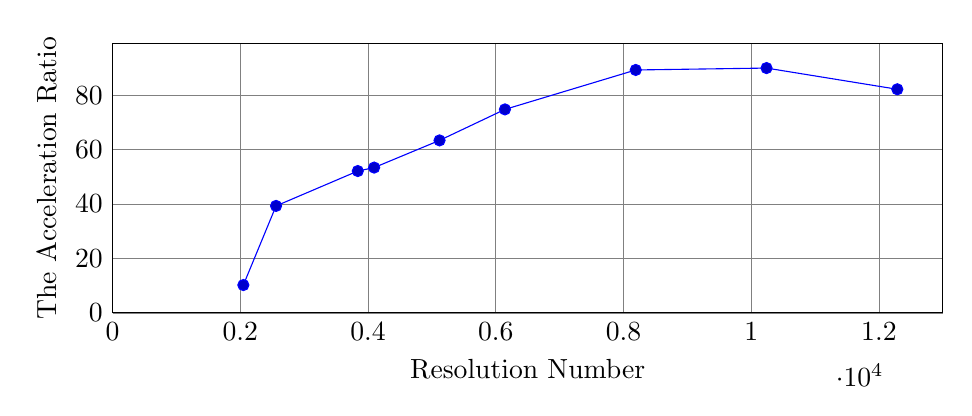
\begin{tikzpicture}
    \begin{axis}[
      width=1\linewidth,
      height=5cm,
      ylabel={The Acceleration Ratio},
      xlabel={Resolution Number},
      grid=major, 
      ymin=0,
      xmin=0,
      xmax=13000,
      grid style={help lines},
    ]

    \addplot coordinates {
(	2048	,	10.2	)
(	2560	,	39.3	)
(	3840	,	52.13	)
(	4096	,	53.4	)
(	5120	,	63.4	)
(	6144	,	74.8	)
(	8192	,	89.3	)
(	10240	,	90	)
(	12288	,	82.2	)


    };
    
    \end{axis}
  \end{tikzpicture}
  \caption{The Acceleration Ratio of Increase in the Speed (Decrease in the Computational Time)}
  \label{t5}
\end{figure}

\clearpage

The ppm image obtained as an output of the code for certain resolution is given in Figure \ref{figure_res_1}. The output picture is the same for both serial code and CUDA implementation as expected. The difference is the time it takes for both to give output individually. 

\begin{figure}[hbt!]
\centering
\begin{subfigure}{0.42\textwidth}
    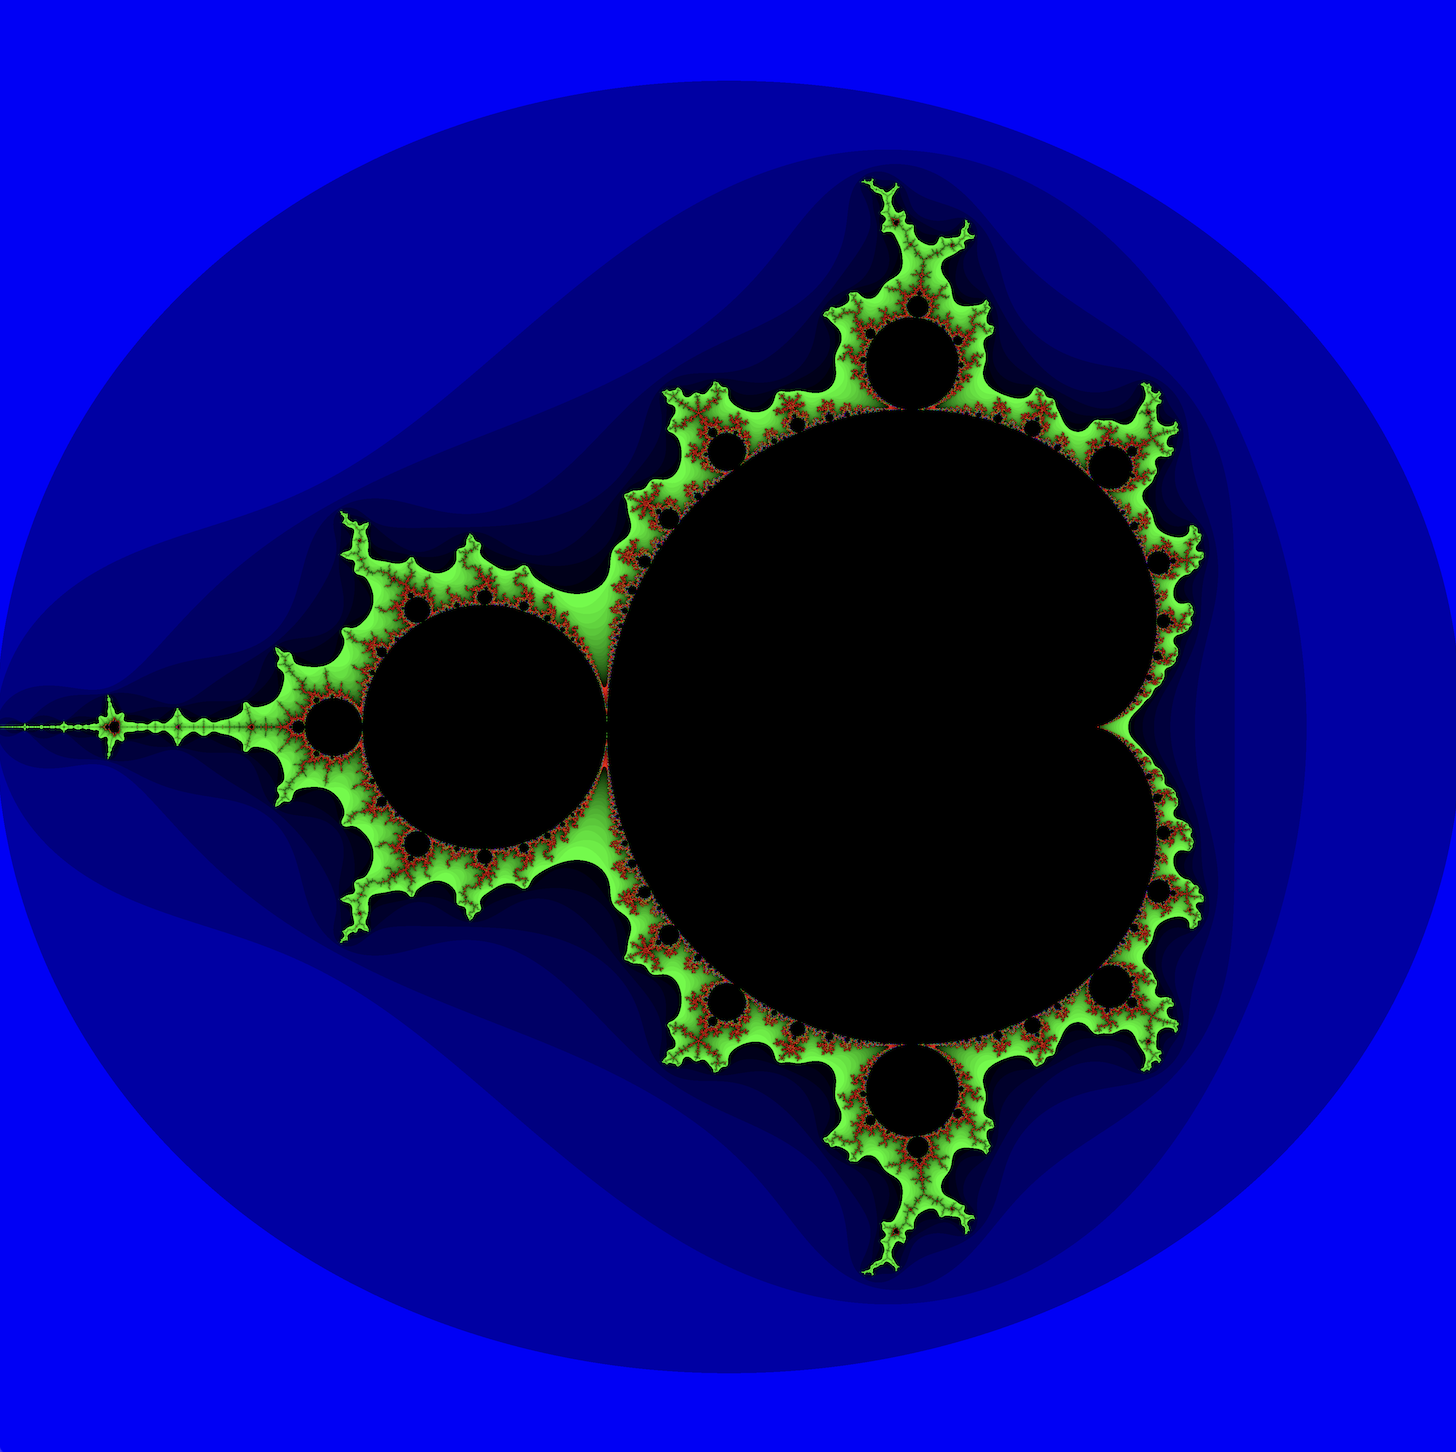
\includegraphics[width=\textwidth]{Figures/serial_4096_4096.png}
\end{subfigure}
\hfill
\begin{subfigure}{0.42\textwidth}
    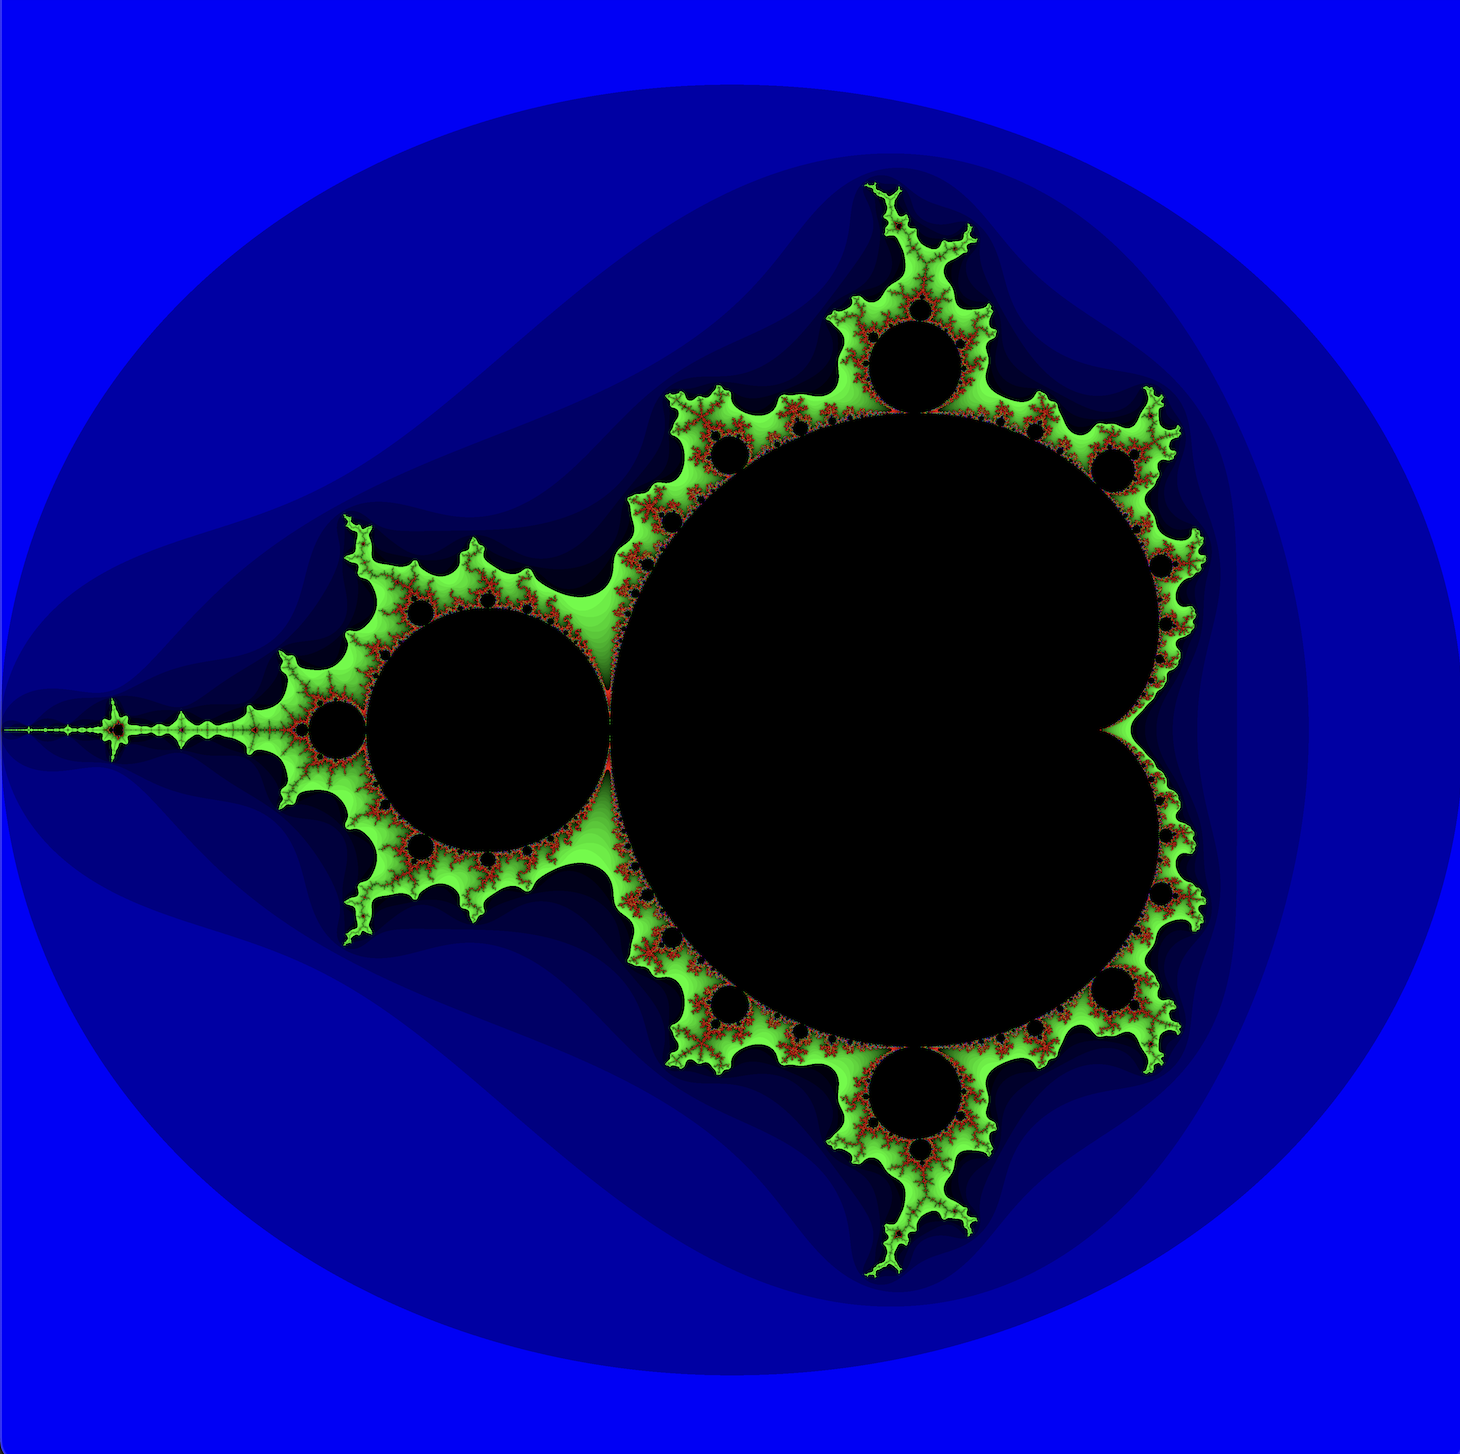
\includegraphics[width=\textwidth]{Figures/paralell_4096_4096.png}
\end{subfigure}
\caption{Left: The output for serial code with 4096 x 4096 resolution. Right: The output for CUDA implementation with 4096 x 4096 resolution.}
\label{figure_res_1}
\end{figure}
\FloatBarrier

\section{Comments and Conclusion}
In this work, we carried out a thorough investigation of the GPU base parallelized mandelbrot set fractal calculator using CUDA. The study concentrated on evaluating the effect of resolution number on CPU-GPU computing time and resolution number on acceleration ratio.  

The calculation time always increases with increasing resolution. However, this can be clearly seen that GPU computation is much much faster than CPU calculation. Moreover, the acceleration ratio is also increasing with increasing resolution resolution. 

In conclusion, our results provide valuable insights into the behavior of the parallelized CUDA solver. 



\clearpage
\printbibliography
\end{document}
